\chapter{lineær programmering}

\begin{comment}
Ting til retter
- bør "def 5.5 mulige løsninger og den mulige mængde" komme før "standard maksimums- og minimumsproblemer"?
- Jeg er ikke sikker på alle termer i dette afsnit. Jeg rettede kriteriefunktion til objektfunktion, da der blev brugt objektfunktion i projektforslaget.
- Jeg er lidt inkonsistent med anvendelsen af [1 2 3] og [1,2,3]. er ikke helt sikker på hvad der ser bedst ud.
- Er der brug for at skrive betingelserne og objektfunktionen ud i starten, eller er det nok at det skrives som vektor-vektor produkt?
\end{comment}

Lineær programmering er en anvendelse af lineær algebra til at finde den optimale resultat af et optimeringsproblem. Lineære programmeringsproblemer tager udgangspunkt i maksimering eller minimering af en lineær funktion. For variablene er der fastsat en række af betingelser, som begrænser de mulige løsninger til problemet.



Funktionen, som ønskes optimeret, kaldes \textbf{objektfunktionen}, og findes på formen:
\begin{align}
f(x_1,x_2,\cdots , x_n)\ =\ c_1x_1 + c_2x_2 + \cdots + c_nx_n = \vec{c}^T \vec{x},
\end{align}
hvor $\vec{x}= \rvect{x_1 & x_2 & \cdots & x_n}^T$ og $\vec{c}= \rvect{c_1 & c_2 & \cdots & c_n}^T$.

Dertil tilføjes en række af betingelser for variablene. Betingelser, som definerer at en variabel er positiv, kaldes en \textbf{positivitetsbetingelse}. 
\begin{align}
	x_i \geq 0
\end{align}
Andre lineære betingelser for variablene kaldes for \textbf{lineære bibetingelser}, og findes på formen, 
\begin{align}
	a_{i,1} x_1 + a_{i,2} x_2 + \cdots + a_{i,n} x_n =\vec{a}_i\vec{x} \ (\leq,=,\geq) \  b_i, \quad \text{for} \ i \in \{1,2,\cdots, m\},
\end{align}
hvor $m$ er antallet af lineære bibetingelser. I en lineær bibetingelse kan venstresiden være begrænset med $\leq, \geq$ eller $=$ i forhold til konstanten $b_i$. I nogle typer af programmeringsproblemer anvendes kun en enkelt af disse relationer. Positivitetsbetingelser er et specialtilfælde af de lineære bibetingelser, da en positivitetsbetingelse blot kan ses som en lineær bibetingelse hvor en koefficient er 1 mens resten er 1 og hvor $b_i=0$.

En \textbf{mulig løsning} til en vektor $\vec{x}$, som overholder alle problemets betingelser.

Et eksempel på et lineært programmeringsproblem ses i Eksempel \ref{eks:maksprob1}. Eksemplet er et lineært maksimeringsproblem, da objektfunktionen søges maksimeret.

\begin{eks}
Et eksempel på et lineært programmeringsproblem ses her, hvor funktionen $f(x_1,x_2)=4x_1+3 x_2$ skal maksimeres.
\begin{center}
\begin{tabular}{l	>{$}r<{$}	>{$}r<{$}	>{$}l<{$}}
Maksimer 		& 		4x_1&	+3 x_2	& \\
med hensyn til 	&  \ \ 	2 x_1& 	- 4 x_2	& \geq - 8\\
				&  		x_1& 	+3 x_2	& \leq 16\\
				&  \ \ 	x_1& 			& \leq 10\\
og $x_2\geq 0$
\end{tabular}
\end{center}

Mængden af alle mulige løsninger til problemet kan vises grafisk. De mulige løsninger findes inden for det grå område på Figur \ref{fig:maksprob1}, hvor $x_1$ og $x_2$ vises henholdsvis på 1. og 2. aksen.

\begin{center}
	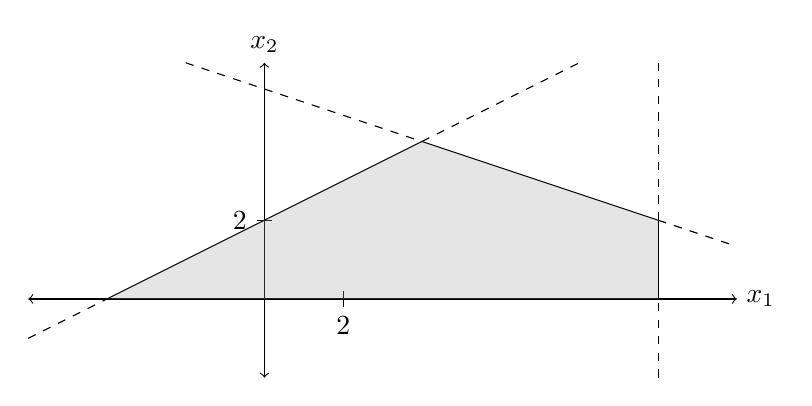
\begin{tikzpicture}
  %laver Grid
  	%\draw[thin,gray!40] (-3,-1) grid (6,3); 
  %x-aksen
  	\draw[<->] (-3,0)--(6,0) node[right]{$x_1$}; 
  %y-aksen
  	\draw[<->] (0,-1)--(0,3) node[above]{$x_2$};
  	
  %akse-markeringer
  	%\node[left] (xakse) at (0,1) {2};
  	\draw[] (-0.1,1) -- (0.1,1) node[pos=0,left] {2};
  	\draw[] (1,-0.1) -- (1,0.1) node[pos=0,below] {2};
  	
  %ligning 1
	\draw[domain=-3:-2,variable=\x,dashed] 	plot({\x},{0.5*\x+1});
	\draw[domain=-2:2,variable=\x] 			plot({\x},{0.5*\x+1});
	\draw[domain=2:4,variable=\x,dashed] 	plot({\x},{0.5*\x+1});
	
  %ligning 2
  	\draw[domain=-1:2,variable=\x,dashed] 	plot({\x},{-(1/3)*\x+8/3});
	\draw[domain=2:5,variable=\x] 			plot({\x},{-(1/3)*\x+8/3});
	\draw[domain=5:6,variable=\x,dashed] 	plot({\x},{-(1/3)*\x+8/3});
	

  %ligning 3
  	\draw[domain=-1:0,variable=\y,dashed] 	plot({5},{\y});
	\draw[domain=0:1,variable=\y] 			plot({5},{\y});
	\draw[domain=1:3,variable=\y,dashed] 	plot({5},{\y});

  %løsningsmængden skraveret
	\fill[gray!80,nearly transparent] (-2,0) -- (2,2) -- (5,1) --(5,0) --  cycle;
\end{tikzpicture}
	\captionof{figure}{Grafisk repræsentation af mulige løsninger.}
	\label{fig:maksprob1}
\end{center}

\label{eks:maksprob1}
\end{eks}

\section{Standard maksimums- og minimumsproblemer}
I et standard maksimumsproblem gælder det for alle bibetingelserne, at den lineære funktion af variablene er mindre end eller lig en konstant, samt at alle variablene er positivt begrænsede.

Som beskrevet i Afsnit \ref{afsnit:lign_sys} kan et lineært ligningssystem opskrives med et matrix-vektor produkt. Tilsvarende gælder det for objektfunktionen, at denne kan skrives som et produkt af to vektorer. Det tillader derved definitionen af standard maksimum problemet med disse produkter i definition \ref{def:std_maks}

\begin{defn}[Standard maksimum problem]
	Lad $\vec{x}= [x_1, x_2,\cdots, x_n]^T$ være \textbf{løsningsvektoren}, med koefficienter $\vec{c}= [c_1, c_2,\cdots, c_n]^T$ i objektfunktionen, og lad $mxn$ matrixen $A=[A_{ij}]$ for $i=1,2,\cdots,m$ og $j=1,2,\cdots,n$ være begrænset af konstanterne $\vec{b}=[b_1, b_2,\cdots, b_m]^T$.
	Da er standard maksimum problemet defineret som\\
\begin{center}
\begin{tabular}{l	>{$}l<{$}}
Maksimer 		& \vec{c}^T\vec{x} \\
med hensyn til 	& A\vec{x} \leq \vec{b}\\
og 				& \vec{x} \geq \vec{0}
\end{tabular}
\end{center}
\label{def:std_maks}
\end{defn}

\begin{defn}[Standard minimum problem]
	Lad $\vec{y}= [y_1, y_2,\cdots, y_m]^T$ være \textbf{løsningsvektoren}, med koefficienter $\vec{b}= [b_1, b_2,\cdots, b_m]^T$ i objektfunktionen, og lad $mxn$ matrixen $A=[A_{ij}]$ for $i=1,2,\cdots,m$ og $j=1,2,\cdots,n$ være begrænset af konstanterne $\vec{c}=[c_1, c_2,\cdots, c_n]^T$.
	Da er standard minimum problemet defineret som\\
\begin{center}
\begin{tabular}{l	>{$}l<{$}}
Minimer			& \vec{y}^T\vec{b} \\
med hensyn til 	& \vec{y}^TA \geq \vec{c}^T\\
og 				& \vec{y} \geq \vec{0}
\end{tabular}
\end{center}
\label{def:std_min}
\end{defn}

\subsection{Omskrivning mellem ligheder og uligheder}
Da et programmeringsproblem ikke nødvendigvis er på den rigtige form fra start, er det vigtigt at kunne omskrive mellem uligheder og ligheder.\\
Omskrivning mellem uligheder
\begin{align*}
	\vec{a}_i\vec{x} \geq b_i \quad \Leftrightarrow \quad -\vec{a}_i\vec{x} \leq -b_i
\end{align*}
Omskrivning fra lighed til ulighed
\begin{align*}
	\vec{a}_i\vec{x} = b_i \quad \rightarrow \quad 	& \vec{a}_i\vec{x} \leq b_i \\
										& \vec{a}_i\vec{x} \geq b_i \\
\end{align*}
Omskrivning fra ulighed til lighed\\
En ulighed kan omskrives til en lighed ved indførslen af en ikke-negativ slack-variabel, som udgør forskellen mellem $\vec{a}_i\vec{x}$ og $b_i$ i uligheden. For maksimeringsproblemer får denne variabel en koefficient på 1 i koefficientmatricen (?) og -1 for minimeringsproblemer. \\
Et standard maksimeringsproblem kan derved omskrives til ligheder ved at indføre en slackvariabel $x_{n+i}$ for hver bibetingelse. Derved bliver betingelserne for henholdsvis et maksimeringsproblem og et minimeringsproblem omskrevet til:
\begin{align*}
	A' &=\rvect{A & I_m}\\
	A' &=\rvect{A & -I_m}
\end{align*}



\begin{eks}[Standard maksimum problem]
Hvis eksempel \ref{eks:maksprob1} skal omskrives til et standard maksimum problem, skal alle uligheder i bibetingelserne være $\leq$. Bibetingelse nr.3 skal derved omskrives. Dette kan gøres ved at gange begge sider af uligheden med $-1$, da dette vender ulighedstegnet. Derudover skal også $x_1$ skal være positivt begrænset. Derved bliver Eksempel \ref{eks:maksprob1} omskrevet til et standard maksimum problem til\\
\begin{center}
\begin{tabular}{l	>{$}r<{$}	>{$}r<{$}	>{$}l<{$}}
Maksimer 		& 		4x_1	&	+3 x_2	& \\
med hensyn til 	&  \ \ 	-2 x_1	& 	4 x_2	& \leq 8\\
				&  		x_1		& 	+3 x_2	& \leq 16\\
				&  \ \ 	x_1		& 			& \leq 10\\
og $x_1 \geq 0, x_2\geq 0$.
\end{tabular}
\end{center}

\begin{center}
	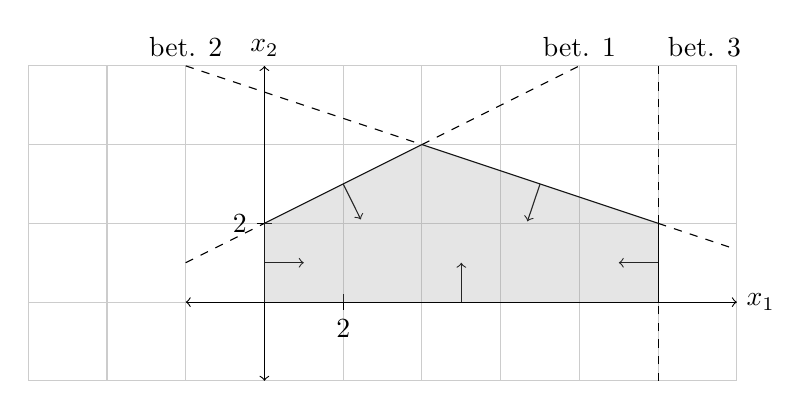
\begin{tikzpicture}
  %laver Grid. godt til når koordinater skal redigeres
  	\draw[thin,gray!40] (-3,-1) grid (6,3); 
  %x-aksen
  	\draw[<->] (-1,0)--(6,0) node[right]{$x_1$};
  	\draw[->] (2.5,0) -- (2.5,0.5);
  %y-aksen
  	\draw[<->] (0,-1)--(0,3) node[above]{$x_2$};
  	\draw[->] (0,0.5) -- (0.5,0.5);
  	
  %akse-markeringer
  	%\node[left] (xakse) at (0,1) {2};
  	\draw[] (-0.1,1) -- (0.1,1) node[pos=0,left] {2};
  	\draw[] (1,-0.1) -- (1,0.1) node[pos=0,below] {2};
  	
  %ligning 1
	\draw[domain=-1:0,variable=\x,dashed] 	plot({\x},{0.5*\x+1});
	\draw[domain=0:2,variable=\x] 			plot({\x},{0.5*\x+1});
	\draw[domain=2:4,variable=\x,dashed] 	plot({\x},{0.5*\x+1}) node[above] {bet. 1};
  	\draw[->] (1,1.5) -- (1.224,1.05);
	
  %ligning 2
  	\draw[domain=-1:2,variable=\x,dashed] 	plot({\x},{-(1/3)*\x+8/3}) node[above] at (-1,3) {bet. 2} ;
	\draw[domain=2:5,variable=\x] 			plot({\x},{-(1/3)*\x+8/3});
	\draw[domain=5:6,variable=\x,dashed] 	plot({\x},{-(1/3)*\x+8/3});
	\draw[->] (3.5,1.5) -- (3.34,1.026);

  %ligning 3
  	\draw[domain=-1:0,variable=\y,dashed] 	plot({5},{\y});
	\draw[domain=0:1,variable=\y] 			plot({5},{\y});
	\draw[domain=1:3,variable=\y,dashed] 	plot({5},{\y}) node[above right] {bet. 3};
	\draw[->] (5,0.5) -- (4.5,0.5);

  %løsningsmængden skraveret
	\fill[gray!80,nearly transparent] (0,0) -- (0,1) -- (2,2) -- (5,1) --(5,0) --  cycle;
\end{tikzpicture}
	\captionof{figure}{Den mulige mængde af et standard maksimeringsproblem.}
	\label{fig:maksprob2}
\end{center}
\label{eks:maksprob2}
\end{eks}

\section{Løsninger til linære programmeringsproblemer}

Den mulige løsningsmængde er mængden af løsningsvektorer, $\vec{x}$, som opfylder alle problemets betingelser. Derved vil den optimale løsning være indeholdt i denne mængde, så længe at mængden ikke er tom.

\begin{defn}[Mulige løsninger og den mulige mængde]
En \textbf{mulig løsning} er en løsningsvektor $\vec{x}$, som opfylder alle problemets betingelser.\\
\textbf{Den mulige mængde} $\mathds{F}$ \textit{(usikker på oversættelsen)} er mængden af alle de mulige løsninger.
\begin{align*}
\mathds{F}=\{\vec{x} \in \mathds{R}|A\vec{x} \leq \vec{b}, \vec{x} \geq \vec{0}\}
\end{align*}
En vektor $\vec{x}$ kaldes en \textbf{optimal løsning}, hvis $f(\vec{x})=\max\limits_{x \in \mathds{F}}f(\vec{x}).$\\
Et problem kaldes \textbf{inkonsistent} (usikker på oversættelse) hvis den mulige mængde er den tomme mængde, ellers er problemet \textbf{konsistent}. Et problem kaldes \textbf{ubegrænset}, hvis objektfunktionen kan tage arbitrært store funktionsværdier for maksimeringsproblemer, og arbitrært små funktionsværdier for minimeringsproblemer. Ellers kaldes problemet \textbf{begrænset}.
\end{defn}

Den optimale løsning kan findes på forskellige måder heriblandt med simplex-metoden, som beskrives i senere kapitler. En anden måde er ved geometrisk visualisering af den mulige mængde. Denne metode er mulig for problemer med op til 3 variable, da løsningsmængden derved visualiseres som et plot i det tilsvarende antal dimensioner. 

\subsection{niveaukurver}
Niveaukurver dannes ved fastsættelsen af funktionsværdi $z=\vec{c}^T \vec{x}$. Niveaukurven er derved mængden af alle vektorer $\vec{x}$, som løser ligningen. Da målet er at maksimere $z$, er målet at finde den største $z$ for hvilken niveaukurven har en ikke-tom skæring med den mulige mængde. dette kan ses i Eksempel \ref{eks:maksprob3}.


\begin{eks}[Optimal løsning fundet grafisk]
Niveaukurverne $46=\vec{c}^T \vec{x}$ og $25=\vec{c}^T \vec{x}$ er på figur \ref{fig:maksprob3} indtegnet for programmeringsprogblemet fra Eksempel \ref{eks:maksprob2}.

	\begin{center}	
		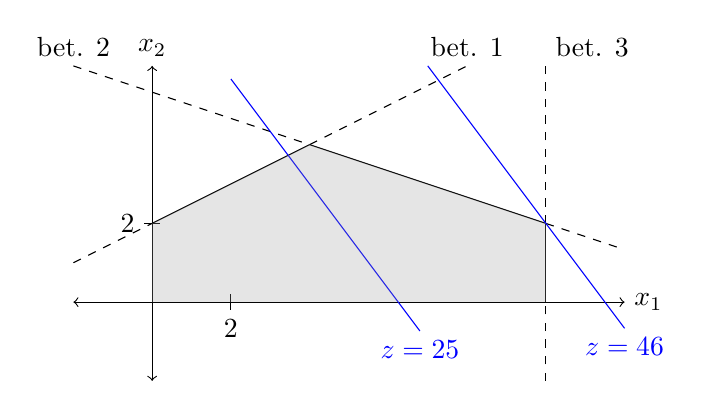
\begin{tikzpicture}
  %laver Grid. godt til når koordinater skal redigeres
  	%\draw[thin,gray!40] (-3,-1) grid (6,3); 
  %x-aksen
  	\draw[<->] (-1,0)--(6,0) node[right]{$x_1$}; 
  %y-aksen
  	\draw[<->] (0,-1)--(0,3) node[above]{$x_2$};
  	
  %akse-markeringer
  	%\node[left] (xakse) at (0,1) {2};
  	\draw[] (-0.1,1) -- (0.1,1) node[pos=0,left] {2};
  	\draw[] (1,-0.1) -- (1,0.1) node[pos=0,below] {2};
  	
  %ligning 1
	\draw[domain=-1:0,variable=\x,dashed] 	plot({\x},{0.5*\x+1});
	\draw[domain=0:2,variable=\x] 			plot({\x},{0.5*\x+1});
	\draw[domain=2:4,variable=\x,dashed] 	plot({\x},{0.5*\x+1}) node[above] {bet. 1};
	
  %ligning 2
  	\draw[domain=-1:2,variable=\x,dashed] 	plot({\x},{-(1/3)*\x+8/3}) node[above] at (-1,3) {bet. 2} ;
	\draw[domain=2:5,variable=\x] 			plot({\x},{-(1/3)*\x+8/3});
	\draw[domain=5:6,variable=\x,dashed] 	plot({\x},{-(1/3)*\x+8/3});
	

  %ligning 3
  	\draw[domain=-1:0,variable=\y,dashed] 	plot({5},{\y});
	\draw[domain=0:1,variable=\y] 			plot({5},{\y});
	\draw[domain=1:3,variable=\y,dashed] 	plot({5},{\y}) node[above right] {bet. 3};
	
  %niveaukurver
  	\draw[domain=3.5:6,variable=\x,blue] plot({\x},{-(4/3)*\x+23/3}) node[below] {$z=46$};
  	\draw[domain=1:3.4,variable=\x,blue] plot({\x},{-(4/3)*\x+25/6}) node[below] {$z=25$};
  	
  %c-vektor
  	%\draw[->,thick,red] (0,0) -- (2,1.5);

  %løsningsmængden skraveret
	\fill[gray!80,nearly transparent] (0,0) -- (0,1) -- (2,2) -- (5,1) --(5,0) --  cycle;
\end{tikzpicture}
		\captionof{figure}{Optimal løsning fundet grafisk}
		\label{fig:maksprob3}
	\end{center}
	
På figuren ses det at den største funktionsværdi $z=46$ findes i skæringen mellem bibetingelse 2 og 3.
Ved at løse bibetingelse 2 og 3 som 2 ligninger med 2 ubekendte findes det at den optimale løsning er $\vec{x}=\rvect{10 & 2}^T.$
\label{eks:maksprob3}
\end{eks}


\begin{comment}
Stadig to do i afsnittet\\
%- infeasible og unbounded tilfælde\\
%- niveaukurver\\
- Hvis der findes en løsning, findes der en optimal løsning (med evt. bevis. burde ikke være så svært med modstrid)\\

Skal jeg have det med at løsninger findes i hjørner? det virker til at kræve en smule mere geometri og hører nok bedre til i geometri afsnittet.
\end{comment}
